%\documentclass[twocolumn,showpacs,preprintnumbers,amsmath,amssymb]{revtex4}
%\documentclass[preprint,showpacs,preprintnumbers,amsmath,amssymb]{revtex4}
\documentclass[amsmath,amssymb]{revtex4}
%\documentclass{article}

% Some other (several out of many) possibilities
%\documentclass[preprint,aps]{revtex4}
%\documentclass[preprint,aps,draft]{revtex4}
%\documentclass[prb]{revtex4}% Physical Review B

\usepackage{algorithm}
\usepackage{algpseudocode}
\usepackage{graphicx}% Include figure files
%\usepackage{dcolumn}% Align table columns on decimal point
%\usepackage{bm}% bold math

%\nofiles

\begin{document}

%\author{}
% \altaffiliation[Also at ]{Physics Department, XYZ University.}
%\author{Second Author}%
% \email{Second.Author@institution.edu}
%\affiliation{%
%Authors' institution and/or address\\
%This line break forced with \textbackslash\textbackslash
%}%
%\author{Charlie Author}
% \homepage{http://www.Second.institution.edu/~Charlie.Author}
%\affiliation{
%Second institution and/or address\\
%This line break forced% with \\
%}%
%\preprint{APS/123-QED}
%\pacs{Valid PACS appear here}
%\keywords{Suggested keywords}
\date{\today}
\title{Bayesian inference of neural connectivity in a population of neurons from 
calcium imaging data.}
\begin{abstract}
We present Bayesian framework for inferring connectivity in a network
of coupled neurons, observed simultaneously using calcium imaging.
\end{abstract}
\maketitle

\section{\label{sec1}Motivation}
The problem of reconstructing connectivity in neural circuits in the brain has recently gained much attention \cite{Hagmann2008,Hagmann2007,Helmstaedter2009,DenkHorstmann04,Briggman2006,Ikegaya2005}. In particular, amid growing evidence of the importance of collective effects in neural networks \cite{Rabinovich2008,Broome2006,Jones2007}, the problem of understanding neural substrates of behavior and cognition via the structure of neural circuits had gradually moved into the spotlight of neuroscience research \cite{Averbeck2008,deBono2005,Song2005,Dunn2004,Chalasani2007,Gray2005,rswormatlas,White1986}.

Traditionally, one is interested in recovering the structure of neural circuit in the form of a wiring diagram specifying the list of synaptic connections in a particular population of neurons alongside with the synaptic connections' strengths and types.
Few different approaches for such comprehensive reconstruction of neural circuits had been proposed in the past including serial section electron microscopy \cite{Briggman2006,Helmstaedter2009}, diffusion tensor imaging \cite{Hagmann2007,Hagmann2008}, ensembles of fluorescent tracers \cite{Bohland2009}, and others.
Electron microscopy remains the standard for neuroanatomical circuits reconstruction with example of complete nervous system reconstruction in C. {\em elegans} available in the literature \cite{White1986,rswormatlas}.
Electron microscopy, however, is known to be extremely expensive, slow and laborious method - reconstruction of the above mentioned circuit with only 300 neurons and fewer than $10^4$ connections took over a decade to complete.
Even with recent developments in automated data acquisition \cite{DenkHorstmann04} and image-processing \cite{Mishchenko2009c,Jain2007,Jurrus2006}, electron microscopy remains an approach limited by long imaging times and extreme vulnerability to errors in neural tracing and image analysis.
Diffusion tensor imaging \cite{Hagmann2007} and ensembles of fluorescent tracers \cite{Bohland2009} potentially offer a technique capable of much faster reconstructions and much larger circuits (also in live subjects in diffusion tensor imaging). However, low resolution of these techniques limits them to only the highest-level information about neural circuit organization, forgoing the fine details of neural connectivity.
Although recently suggested method for collating information from ensembles of fluorescent markers using Compressive Sensing \cite{Mishchenko2009a,Mishchenko2009} may allow to overcome both the speed limitation of electron microscopy and resolution limit of optical techniques, this method requires development of novel genetic constructs and may be challenging to scale up to larger circuits.
Overall, the problem of large scale reconstructions of the structure of neural circuits using neuroanatomy approach remains extremely challenging endeavor.


Another family of methods for inferring neural connectivity is using observations of neural activity in population of neurons, such as micro-electrodes recordings of external field potential
\cite{Meister1994,Litke2003,Litke2004,PILL07,Stevenson2008} or functional magnetic resonance imaging (fMRI) [NEED REF].
Unlike the neuroanatomy approach, these techniques illuminate the structure of neural circuits in terms of their functional connectivity.
Functional connectivity may be defined as the statistical effect one neuron's activity has upon another, i.e. two neurons are functionally connected if their spike trains are conditionally dependent given all the other observable variables, including the stimulus and the activity of all other neurons.
Although details of the relationship between functional connectivity and anatomical circuit structure are yet to be elaborated, empirical knowledge of functional connectivity is important both fundamentally and for applications. Immediate knowledge of both functional and anatomical connectivity may be required to elucidate the relationship between the two, and also functional connectivity provides access to invaluable information about coding and decoding of signals in neural populations necessary for applications such as neural interfaces or neuro-prosthetics.

Despite their numerous advantages and many applications, both micro-electrode recordings and fMRI have also serious limitations. In case of external field recordings, application of this approach are limited by the size of largest micro-electrode arrays restricting the largest size of neural population that can be observed. Neural population with only $\leq 100$ cells can be simultaneously observed in state of the art experiments. fMRI, although potentially giving fast access to the entire brain in in-vivo conditions, is constrained by bad spatial and temporal resolution of fMRI signal, and uncertain relationship of fMRI signal (i.e. blood flow) with the neural activity.

Recently, great advances in the development of calcium indicators, delivery techniques, and microscopy technologies have facilitated calcium imaging of neural activity of large populations of neurons in a wide array of neural substrates \cite{Ikegaya2005,Nagayama2007,Nevian2007,Gobel07b}. Calcium imaging is an excellent tool for collecting large-scale data for functional connectivity, and is potentially capable of overcoming both the resolution limits of fMRI and population size limit of multi-electrode arrays. With calcium imaging, recordings at the level of individual cells are possible for thousands and tens of thousands of cells while retaining resolution sufficient for reconstruction of individual spikes \cite{Ikegaya2005}. In this paper we develop a Bayesian formalism for inferring neural connectivity in a population of neurons from such calcium imaging data.

\section{\label{sec:methods}Methods}
\subsection{\label{sec:methods:introduction}Overview}
\begin{table}[h!b!p!]
\begin{tabular}{ll}
Number of neurons         & $N$ \\
Calcium imaging duration & $T$ \\
Single neuron spike & $n_i(t)$ \\
Single neuron calcium concentration & $C_i(t)$ \\
Single neuron state & $X_i(t)=(n_i(t),C_i(t))$ \\
Sequence of neural states & $X_i=\{X_i(t),t=1\ldots T\}$ \\
Fluorescence observation from single neuron & $F_i(t)$ \\
Sequence of fluorescence observations & $F_i=\{F_i(t),t=1\ldots T\}$ \\
Set of spike-trains from all neurons   & ${\bf X}=\{X_i\}$ \\
Set of fluorescence observations from all neurons & ${\bf F}=\{F_i\}$ \\
Functional connection weights & $w_{ij}(t)$ \\
Matrix of all connection weights & $W=\{w_{ij}(t)\}$ \\
Calcium dynamics model for single neuron & $M_i$ \\
Calcium dynamics model for all neurons & $M=\{M_i\}$
\end{tabular}
\caption{Table of notations. Indices $i,j=1\ldots N$ refer to the neurons in the population. Bold notation is used to represent the vector states over all neurons, e.g. ${\bf X}=\{X_i,i=1\ldots N\}$. Whenever $t$ is dropped for brevity the entire sequence $t=1\ldots T$ is implied, e.g. ${\bf X}=\{{\bf X}(t),t=1\ldots T\}$.}
\label{table:notation}
\end{table}
Our goal is to evaluate connectivity in a population of neurons observed with calcium imaging.
Calcium imaging is experimental technique for monitoring neuron's electrical activity  by observing the concentration of calcium inside the cell. 
Calcium concentration under normal conditions fluctuates around some background level. 
However, when the neuron issues a spike, influx of calcium ions from outside of the cell causes its concentration to spike instantaneously. 
Spikes of individual neurons, thus, may be detected remotely by monitoring calcium level inside cells with fluorescent dyes sensitive to calcium concentration (i.e. changing brightness $F$ in proportion to calcium concentration, see Figure \ref{fig:egfluor} for example).

Most of the calcium indicators, however, are very slow with the relaxation time of calcium concentration on the order of 100 ms. Thus, monitoring intracellular calcium concentration has been commonly used in neuroscience to make conclusions about the overall activity state of neural cell, e.g. high activity, medium activity, without reference to individual spikes.
However, under appropriate conditions  calcium imaging allows not only to make conclusions about such general levels of activity, but also to recover entire spike trains of neural cell with remarkable precision \cite{Vogelstein2009}.
Recovering accurate spike trains for a population of neurons interacting via a set of synapstic connections, in turn, gives access to inferring functional connectivity in such populations by directly correlating spike-trains of different neurons.

Formally, functional connectivity may be described as a matrix of functional connection weights $w_{ij}(t-t')$, each representing the conditional change in the probability for neuron $i$ to fire at time $t$ given neuron $j$ had fired at some time $t'$ before given all other available variables.
Recovery of such matrix of functional connection weights $W=\{w_{ij}\}$ from the set of fluorescence observations ${\bf F}=\{F_i\}$, acquired with calcium imaging, is the primary goal of this work.


\subsection{\label{sec:methods:markov-setup}Hidden Markov Model for calcium imaging of neural population}
In this work neural activity of a population of neurons is modeled with the standard generalized linear model (GLM), which is known to capture well the statistical properties of the firing of individual neurons \cite{PILL07,PAN03d,Wu07,Rigat06,OKA05},
\begin{equation}\label{eqn:glm:definition}
\begin{array}{l}
n_i(t)\sim \text{Bernoulli}(\lambda_i(t)\Delta), \\
\lambda_i(t)=f(J_i(t))=f(b_0^i+k_i\cdot S^{ext}(t)+\sum\limits_{j=1}^{j=N} \sum\limits_{t'<t} w_{ij}(t-t')n_{j}(t')).
\end{array}
\end{equation}
($ 0 < \lambda_i(t)\Delta<1$)
Here, the spiking of neurons is described as a stochastic Bernoulli process driven by external stimulus $S^{ext}(t)$ as well as the activity of other neurons in the population ${\bf n}=\{n_{j}(t)\}$, connected to each other via synapses $w_{ij}$.
$\lambda_i(t)$ is instantaneous firing rate of neuron $i$, $b_0^i$ and $k_i\cdot S^{ext}(t)$ are the baseline and the external stimulus terms, respectively, and $\Delta$ is the time step.
In this paper we are concerned with studying spontaneous activity in a population of neurons, thus the external stimulus term $S^{ext}(t)$ from now on will be dropped.
Parameters $w_{ij}(t)$ describe functional couplings between neurons and correspond to the functional connectivity in GLM.
The rate-function $f(J)$ is exponential, $f(J)=\exp(J)$. 
This choice is motivated by significant computational simplifications when estimating GLM parameters, 
by making MAP estimation problem convex - an important advantage for working with large volumes of data
in neural activity recordings \cite{PAN03d}.

If actual neural spikes $n_i(t)$ were directly observed, the problem of estimating functional connectivity from a set of observed spike trains would have reduces to a known problem such as in \cite{PILL07}. With calcium imaging, however, we do not directly observe spike trains. Instead, fluorescent signal from the calcium-reporter couples with the neural activity via hidden nonlinear calcium dynamics \cite{Vogelstein2009},
\begin{equation}\label{eqn:ca:definition}
\begin{array}{l}
C_i(t) = C_i(t-1) + (C^i_b-C_i(t-1)) \Delta/\tau^i_c + A^i_c n_i(t)+\epsilon_c^i(t), \\
F_i(t) \sim \text{Poiss}( S(C_i(t);\alpha^i_c,\beta^i_c) ).
\end{array}
\end{equation}
Eq. (\ref{eqn:ca:definition}) describes evolution of intracellular calcium concentration $C_i(t)$ in the neuron $i$ with time $t$. Under normal conditions, the intracellular concentration is fluctuating around the baseline level of $C^i_b$ with normally distributed noise $\epsilon^i_c(t)$ with variance $(\sigma^i_c)^2\Delta$, first two and the last terms.
The third term describes instantaneous jump in the intracellular calcium concentration $A^i_c$ when the neuron fires a spike.
Calcium imaging signal, $F_i(t)$, is described by the count of photons collected at the detector per neural cell per one imaging frame. It is distributed according to Poisson statistics with the mean given by generalized Hill function $S(C)=\alpha^i_c C/(C+K_d) + \beta^i_c$ \cite{Yasuda2004}.

The hierarchical model Eq.(\ref{eqn:glm:definition}) and (\ref{eqn:ca:definition}) is governed by $6N$ calcium dynamics parameters - calcium decay time-constant $\tau_c$, background calcium concentration $C_{b}$, fluctuations in calcium concentration $\sigma_c$, per-spike calcium jump $A_c$, photon budget scaling $\alpha_c$ and background $\beta_c$, which we jointly denote as $M_i=\{\tau^i_c, C^i_{b}, \sigma^i_c, A^i_c, \alpha^i_c, \beta^i_c\}$, and $m N^2 + N$ functional connectivity weights $w_{ij}(t)$ and $b^0_i$ which we jointly denote as $W=\{w_{ij}(t),b_0^i\}$, $m$ is the temporal depth of coupling weights $w_{ij}(t)$.

\subsection{\label{sec:methods:estimating_parameters}Estimating parameters of neural population calcium imaging Hidden Markov Model }
Our goal is to estimate the model parameters, such as $W$ and $M$, given calcium imaging observations ${\bf F}$. A natural approach for such estimation is to obtain MAP estimate of these parameters with
\begin{equation}\label{eqn:MAP}
(M,W)^*=\text{argmax } P(M,W|{\bf F}).
\end{equation}
While we may be unable to calculate the probability $P(M,W|{\bf F})$, our hierarchical model Eqs.(\ref{eqn:glm:definition}) and (\ref{eqn:ca:definition}) allows us to calculate $P({\bf F},{\bf X},M,W)\sim P({\bf F},{\bf X}|M,W)$. A natural approach to solving problem (\ref{eqn:MAP}) then is to use the Expectation Maximization algorithm (EM).
EM allows to obtain MAP estimates of HMM parameters by going through a series of iterations $(M,W)^{(l)}$, each time finding a better approximation to the MAP solution by maximizing the conditional expectation values
\begin{equation}
(M,W)^{(l+1)}=\text{argmax }E_{P({\bf X}|M^{(l)},W^{(l)},{\bf F})}\left[\log P({\bf X},{\bf F},M,W)\right].
\end{equation}

The expectation to be computed in our case is
\begin{equation}\label{eqn:loglik:definition-expl}
\sum_i^N E[\log P_{[Ca]}(F_i|{\bf X},M_i,W)] + \sum_i^N E[\log P_{GLM}(n_i|{\bf n}_{/i},W)].
\end{equation}
Here ${\bf n}_{/i}=(n_1,...,n_{i-1},n_{i+1},...n_N)$, $P_{[Ca]}(F_i|{\bf X},M_i,W)$ is the likelihood of observing signal $F_i$ \cite{Vogelstein2009}, and $P_{GLM}$ likelihood can be calculated from Eq.(\ref{eqn:glm:definition}),
\begin{equation}\label{eqn:likelihoodGLM-expl}
\begin{array}{l}
E\left[\log P_{GLM}(n_i|{\bf n}_{/i},W\right]=\sum\limits_t E \left[ n_i(t) J_i(t)\right] - E\left[(1-n_i(t)) \exp(J_i(t)) \Delta \right],\\
J_i(t)=b_0^i+\sum\limits_{j} \sum\limits_{t'<t} w_{ij}(t-t')n_{j}(t'),
\end{array}
\end{equation}
Note that while the first term in Eq.(\ref{eqn:likelihoodGLM-expl}) is simple to compute and only requires $E[n_i(t)]$ and $E[n_i(t) n_{j}(t')]$, the second term does not reduce to simple sufficient statistics. In order to evaluate this expectation value we need to obtain joint sample from the distribution of all spike trains $P({\bf n}|M,W,{\bf F})$.

Given Markovian nature of model Eq.(\ref{eqn:glm:definition}) and (\ref{eqn:ca:definition}), obtaining such sample is an instance of a well known problem of sampling from HMM. In particular, for a finite state-space HMM forward-backward procedure is known to provide samples in  $O(T)$ time \cite{RAB89}. For continuous state-space HMM different sampling strategies exist relying on discretizing the continuous state-space and approximating the integrals in forward-backward procedure using Monte Carlo \cite{DFG01,MINKAPHD,Fearnhead2003,koyama08,Andrieu2007,NBR03}.

In our case, the state $X_i(t)$ is a direct product of binary $n_i(t)$ and continuous $C_i(t)$ dimensions, and so a continuous state-space sampling algorithm is required.
Given large length of neural activity recordings data, $O(T)$ computational cost of HMM sampling algorithms is an important advantage.

One of the most popular methods for sampling from continuous-state HMM is sequential Monte Carlo (SMC), also known as particle filter \cite{DFG01}. In SMC, discretization of the state-space is constructed by drawing a sample from marginal distributions  $P({\bf X}(t)|\{{\bf F}(t'),t'=1\ldots t\})$, computed in the forward pass, and the forward-backward integrals are approximated using Monte Carlo on such samples. The main difficulty of SMC in our case is extremely high dimensionality of the state-space - for a population of $N\sim 50$ neurons, the dimensionality of the state space is $2N\sim 100$. Integrals in forward-backward procedure, therefore, cannot be accurately sampled using particle swarms of tractable size.

To solve this problem, we propose a hybrid SMC-Gibbs sampling strategy taking advantage of the specific structure of the model Eqs.(\ref{eqn:glm:definition}) and (\ref{eqn:ca:definition}), namely, that it can be viewed as a set of $N$ coupled HMM models. Gibbs sampling is a procedure for obtaining samples from high-dimensional distribution $P({\bf X})$ by sampling from low-dimensional conditional distributions $P(X_{i}(t)|{\bf X}_{/i,t})$ one variable $X_{i}(t)$ at a time \cite{Gelfand1990}.  Gibbs sampling allows to reduce intractable high-dimensional sampling problems to sequences of tractable low-dimensional subproblems.
Here, we propose Gibbs sampling in blocks of one neuron sequence $X_{i}$ at a time: if we view the spike-train history ${\bf X}=(X_1,...,X_N)$ as a set of blocks of spike trains from individual neurons $X_i$, we perform Gibbs sampling by consequently sampling such entire blocks $X_i\sim P(X_{i}|{\bf X}_{/i},M,W,{\bf F})$ one at a time.
Note that such block-sampling strategy is necessary here since different $t$ states in $X_i(t)$ for same neuron $i$ are correlated via Markov dynamics, thus leading to slow mixing of Gibbs chain if we Gibbs-sample from $X_i(t)$ for different $t$ and same $i$.
Although each sampling sub-problem in our case is still high-dimensional, it is tractable because it reduces to sampling from HMM with 2D state-space. Thus, joint sample from $2N$-dimensional HMM $P({\bf X}|M,W,{\bf F})$ may be obtained.

Maximization step of EM requires maximizing conditional expectation of $\log P({\bf X},{\bf F},M,W)$ given such sample. In our case, such maximization is a very large optimization problem involving $6N$ parameters $M$ and $mN^2+N$ parameters $W$. Fortunately, special structure of Eq.(\ref{eqn:loglik:definition-expl}) allows to simplify optimization problem dramatically by performing optimization with respect to different neurons $i$ independently.

EM algorithm therefore requires solving following problems: 
sampling individual neuron state-sequences $X_i\sim P(X_{i}|{\bf X}_{/i},M,W,{\bf F})$ using HMM sampling technique,
obtaining joint sample of neuron state-sequences ${\bf X}\sim P({\bf X}|M,W,{\bf F})$ using Gibbs technique,
solving for next iteration of parameters $M$ and $W$ by maximizing conditional expectation value of the log-likelihood $P({\bf X},{\bf F},M,W)$.

\begin{algorithm}
\caption{Pseudocode for estimating functional connectivity from calcium imaging data using EM.}\label{eqn:pseudocode}
\begin{algorithmic}
\While{$|W^{(l)}-W^{(l-1)}|>\text{threshold}_W$}
  \ForAll{$i=1\ldots N$}
    \While{$|M^{(l)}_i-M^{(l-1)}_i|> \text{threshold}_M$}
      \State Sample $X_i \sim P(X_i|{\bf n}_{\i},M_i,W,{\bf F}_i)$
      \State Maximize $M^{(l+1)}=\text{argmax} E\left[\log P_{[Ca]}(X_i,{\bf n}_{\i},M_i,W,{\bf F}_i)|X_i\right]$
    \EndWhile
  \EndFor
  
  \For{$k=1\ldots N_G$}
    \ForAll{$i=1\ldots N$}
      \State Sample $n_i \sim P(n_i|{\bf n}_{/i},M_i,W,{\bf F}_i)$
    \EndFor
  \EndFor 

  \State Maximize $W^{(l+1)}=\text{argmax} E\left[\log P_{GLM}({\bf n}|W)|{\bf n}\right]$  
\EndWhile
\end{algorithmic}
\end{algorithm}

\subsection{\label{sec:methods:sampling_neuron}Sampling individual neuron spike-trains and estimating calcium model parameters $M_i$ using SMC}
JOSH - PF review from \cite{Vogelstein2009}, estimating calcium models.

\subsection{\label{sec:methods:sampling HMM}Sampling joint spike-trains using hybdir MCMC and Gibbs algorithm}
In order to sample spike-train of a neuron from the imaged population, the spike-train may be drawn over the set of particle swarms generated in the forward pass of the particle filter abov using a variant of finite forward-backward procedure.
Such procedure, however, is known to result in biased samples \cite{Andrieu2007,NBR03}.
Specifically, such samples are distributed with the probability density
\begin{equation}
X_i \sim P(X_i(t=1)|{\bf X}_{/i},W)\prod\limits_{t=2}^{t=T-1}P(X_i(t)|X_i(t-1),{\bf X}_{/i},W)\prod\limits_{t=1}^{t=T}P(F_i(t)|X_i(t),M_i)/Z(G),
\end{equation}
where $Z(G)=\sum\limits_{\{X_i(t)\}\in G}P(X_i(t=1)|{\bf X}_{/i},W)\prod\limits_{t=2}^{t=T-1}P(X_i(t)|X_i(t-1),{\bf X}_{/i},W) \prod\limits_{t=1}^{t=T}P(F_i(t)|X_i(t),M^i)$. 
In particular, such probabilities of different sequences differ from the true probabilities by the difference in the estimated normalization constant $Z(G)$ from the true normalization $Z$.
This bias may be removed by embedding SMC into a larger importance sampling algorithm, correcting for bias $Z(G)$ by retaining SMC samples with probability $\sim Z(G)$ \cite{Andrieu2007}. In particular, Andrieu et al. \cite{Andrieu2007} show that as the size of the particle swarm grows the acceptance ratio of such importance sampling tends to unity.

A different and somewhat simpler approach, developed by Neal et al. \cite{NBR03}, is to use Markov Chain Monte Carlo method (MCMC) with the Markov chain constructed specifically to have the necessary equilibrium distribution $P(X_i|M,W,{\bf F})$. The Markov Chain is constructed as follows. First, continuous-state HMM is replaced with a discrete HMM on a grid of points $G=\prod G(t)$, where $G(t) = \{X_i^{(l)}(t), l=1\ldots q\}$, $X_i^{(l)}(t)\sim \rho^i_t(X_i(t))$. I.e., at each time-point $t$ we define a pool of $q$ grid-points $\{X_i^{(l)}(t)\}$ drawn independently from a given proposal density $\rho^i_t(X_i(t))$. The grid $G$ is then constructed as a direct product of such pools.

Second, sequence of states is selected over such grid with the probability
\begin{equation}\label{eqn:nealprob}
X_i\sim P(X_i(t=1)|{\bf n}_{\i},W)\prod\limits_{t=2}^{t=T-1}P(X_i(t)|X_i(t-1),{\bf n}_{\i},W)\prod\limits_{t=1}^{t=T}
\frac{P(F_i(t)|X_i(t),M_i)}{\rho^i_t(X_i(t))}.
\end{equation}
This may be done directly and efficiently using forward-backward procedure with the observation probability modified to $P(F_i(t)|X_i(t),M_i)\rightarrow P(F_i(t)|X_i(t),M_i)/{\rho^i_t(X_i(t))}$.

Finally, states from the chosen sequence of states $X_i$ should be included in the pools $G(t)$ for the next MCMC step, $X_i(t)\in G(t)$, and the above two steps should be repeated with the new grid $G$. It is shown in \cite{NBR03} that the limiting distribution of such Markov chain is the correct unbiased distribution
\begin{equation}
P(X_i(t=1)|{\bf n}_{\i},W)\prod\limits_{t=1}^{t=T-1}P(X_i(t)|X_i(t-1),{\bf n}_{\i},W)\prod\limits_{t=1}^{t=T}P(F_i(t)|X_i(t),M_i).
\end{equation}
The advantage of Neal's method is that the grids $G$ are simple to prepare and also that no importance sampling rejection step is required - such step is implicitly accommodated in the forward-backward procedure via modified observation probability Eq.(\ref{eqn:nealprob}).

Proposal density $\rho^i_t(X_i(t))$ may be chosen arbitrary as long as it has sufficiently large support.
In order to achieve faster convergence, we use marginal densities $P(X_i(t)|{\bf X}_{/i},M,W,{\bf F})$ computed from the conventional SMC algorithm. Such accurate $\rho^i_t(X_i(t))$ allows the Markov Chain to converge extremely quickly.
$\rho^i_t(X_i(t))$ were constructed using kernel density estimation such that $\rho^i_t(C_i(t))$ was a mixture of Gaussians centered on particles from the particle swarm $C_i^{(l)}(t)$ with the variances $\approx var\left[C_i^{(l)}(t)-C_i^{(l')}(t)\right]$. $\rho^i_t(n_i(t))$ was taken to be Bernoulli distribution with the spike probability estimated from the particle swarm. Finally, $\rho^i_t(X_i(t))=\rho^i_t(n_i(t))\rho^i_t(C_i(t))$.

Such spike-train samples for single neurons from the conditional probability distributions $P(X_i|{\bf X}_{/i},M,W,{\bf F})$ may be subsequently used in block-Gibbs sampling procedure to acquire joint sample from $P({\bf X}|M,W,{\bf F})$ for a large number of coupled individual neuron HMM exactly and efficiently.
Specifically, we repeat the MCMC procedure to sample blocks of one neuron state-sequence at a time $X_i\sim P(X_{i}|{\bf X}_{/i},M,W,{\bf F})$ sequentially for all neurons $i=1\ldots N$ for $N_G$ Gibbs cycles. 
We accumulate samples at the end of each of $N_G$ cycles.

A substantial simplification may occur if SNR in the calcium imaging data is high. In this case, the posterior distribution for neural states is dominated by the fluorescence term $P(X_i|*)\approx P(X_i|F_i)$, and the joint distribution for ${\bf X}$ approximately factorizes $P({\bf X}|M,W,{\bf F})\approx\prod P(X_i|F_i,M_i)$. If this factorization is sufficiently accurate, the sample of ${\bf X}$ may be obtained by independently drawing state-sequences for single neurons $X_i \sim P(X_i|F_i,M_i)$ and then combining them to form the joint sample ${\bf X}$.  We refer to such samples as the independent approximation. Depending on the accuracy of such approximation, it may or may not be acceptable for the estimation of functional connectivity matrix $W$ from the calcium imaging data. However, as we show below, it is indeed the case that the independent approximation is adequate here for interesting calcium imaging SNR regimes.

MCMC-Gibbs procedure for sampling joint spike trains above allows to obtain sample of ${\bf n}\sim P({\bf n}|W,M,{\bf F})$ from a high-dimensional HMM. However, if the temporal structure of the functional connection weights $w_{ij}(t)$ is known in advance, e.g. if $w_{ij}(t)=w_{ij}\exp(-t/\tau_w)$, drawing spike-train samples from $P({\bf X}|M,W,{\bf F})$ may be avoided by using marginal distributions of the reduced history variables $P({\bf h}(t)|M,W,{\bf F})$,
\begin{equation}
h_i(t)=\sum\limits_{t'<t} n_i(t')\exp(-(t-t')/\tau_w).
\end{equation}
In terms of $h_i(t)$ GLM likelihood may be written as follows,
\begin{equation}
E[\log P_{GLM}(n_i|{\bf h},W)]\approx \sum_t \left(\sum\limits_{j} w_{ij} E[n_i(t) h_j(t)] -
E[(1-n_i(t)) \exp(\sum\limits_j w_{ij}h_j(t))] \Delta \right),
\end{equation}
so that GLM parameters may be estimated from the marginal distributions $P({\bf n}(t),{\bf h}(t)|M,W,{\bf F})$ without drawing the full spike-train samples ${\bf n}$.

Using reduced history variables provides substantial simplification over full MCMC procedure. In particular, such history variables may be constructed via Markov process
\begin{equation}\label{eqn:spkhist:definition}
h_i(t)=(1-\Delta/\tau_w) h_i(t-1) + n_i(t-1) + \epsilon_i(t),
\end{equation}
where $\epsilon_i(t)$ is additional normally distributed internal noise term with variance $\sigma^2_h$, and so their marginal distributions may be estimated using above particle filter method. If the time-history of the  functional connection weights may be represented as a linear combination of few exponentials with different decay times, Eq.(\ref{eqn:spkhist:definition}) may be obviously generalized to this case to also use multiple reduced history variables $h_i^{(l)}(t)$, each with a different time-constant $\tau^{(l)}_w$, in order to represent such more complex time-dynamics, allowing estimating GLM parameters from marginal distributions $P({\bf n}(t),\{{\bf h}^{(l)}(t)\}|M,W,{\bf F})$.
Such formulation of GLM inference problem is completely equivalent to the above formulation operating with the full spike-train samples ${\bf X}$, and may be used fully interchangeably with it. Given better computational cost of computing marginal distributions $P({\bf n}(t),{\bf h}(t)|M,W,{\bf F})$, in suitable conditions this approach may be extremely advantageous.


\subsection{\label{sec:methods:parameters HMM}Estimating parameters of the Hidden Markov Model}
In order to perform maximization step of EM, the expectation of the log-likehood  Eq.(\ref{eqn:loglik:definition-expl}) needs to be maximized with respect to $M=\{M_i\}$ and $W=\{w_{ij}(t),b_0^i\}$. For $N$ neurons this is a very large optimization problem with $6N$ parameters $M$ and $m N^2 + N$ parameters $W$.
Fortunately, this optimization problem admits dramatic simplifications making it tractable for existing computers.
Specifically, estimation of parameters $M_i$ may be performed individually for each neuron since calcium dynamics of different neurons are independent from each other and, given $H$, also decoupled from GLM. Finding parameters $M_i$, thus, only involves solving of $N$ 6D-optimization sub-problems (see \cite{Vogelstein2009} for details).

Finding GLM parameters is an optimization problem with $mN^2+N$ variables. By construction, however, GLM log-likelihood $P_{GLM}(H,W)$ is convex and, also, GLM log-likelihoods for different neurons, Eq.(\ref{eqn:likelihoodGLM-expl}), are independent and may be maximized separately. Finding parameters $\{w_{ij}(t),b^i_0\}$, thus, only involves solving of $N$ $mN+1$-dimensional convex optimization sub-problems, which can be done efficiently using standard algorithm such as gradient ascent, conjugate gradient or Newton-Rapson methods. E.g., we used standard Matlab's nonlinear optimization function {\em fminunc}, provided in optimization toolbox, to solve this problem for up to $N=500$ neurons.

Simple properties of the connectivity matrix, that may be known a-priory, may be extremely helpful in obtaining accurate solutions for smaller datasets. In particular, enforcing sparseness for signal recovered with a series of linear measurements via $L1$-regularizer is known to dramatically reduce the amount of data necessary to accurately reconstruct the signal \cite{Candes2005,DE03,Mishchenko2009}. Although here the estimation problem is not linear, it is interesting what impact analogous prior might have on the reconstruction of the matrix of functional connection weights $W$.
Enforcing sparseness may be done by introducing exponential prior to GLM \cite{Stevenson2009}, thus leading to the posterior probability for the spike train
\begin{equation}\label{eqn:likelihoodsparseGLM}
E[\log P_{GLM}(n_i|{\bf n}_{/i},W)P(W)]=\sum_t E\left( n_i(t) J_i(t) - (1-n_i(t)) \exp(J_i(t)) \Delta \right)-\lambda \sum_{t'ij}|w_{ij}(t')|.
\end{equation}
Exponential prior parameter $\lambda\sim 1/\langle|w_{ij}|\rangle$ may be set from a-priory neuroanatomical or neurophysiological data.
Sparse prior does not change the convexity of GLM log-likelihood and, so, such regularized problem may be solved efficiently using methods of convex optimization theory.
E.g., by introducing slack variables $s_{ij}(t)>|w_{ij}(t)|$, this problem may be converted to a nonlinear program that can be solved using interior point method
\begin{equation}\label{eqn:conconvexopt}
\begin{array}{l}
\min \left\{-\sum\limits_t E\left[ n_i(t) J_i(t) - (1-n_i(t)) \exp(J_i(t)) \Delta \right]+
\lambda \sum\limits_{t'j}s_{ij}(t')\right\}, \text{ s.t. }\\
w_{ij}(t')<s_{ij}(t'), -w_{ij}(t')<s_{ij}(t') \forall j,t'.
\end{array}
\end{equation}
We used Matlab's standard function {\em fconmin}, provided in optimization toolbox, to solve this constrained optimization problem for up to $N=500$ neurons. As we will see below, sparse prior dramatically decreases the amount of data necessary for accurate estimation of the connectivity matrix.

Another property of the connectivity matrix that may be useful is the so called Dale's law. Dale's law is the empirical observation that neurons always make synapses of one kind, i.e. either inhibitory or excitatory. In terms of the connectivity matrix, Dale's law translates into the condition of sign-constancy of the matrix columns. Dale's law is easy to enforce by constraining $w_{ij}$ to be either positive or negative for given $j$.
Sign assignments may be chosen by inspecting unconstrained solution $W$ and choosing the row $w^{i*}$ to be excitatory if the sum-squares of the positive terms $w_{ij}$ for given $j$ in the unconstrained solution is greater than that of the negative terms, and inhibitory otherwise.
After that, Dale's law may be enforced either independently or together with the sparse prior.
The nonlinear program in the latter case becomes
\begin{equation}
\begin{array}{l}
\min \left\{-\sum\limits_t E\left[ n_i(t) J_i(t) - (1-n_i(t) \exp(J_i(t)) \Delta \right]+\lambda \sum\limits_{t'j}s_{ij}(t')\right\}, \text{ s.t. }\\
w_{ij}(t')<0, -w_{ij}(t')<s_{ij}(t') \forall j,t'\text{ where }j\text{ is inhibitory neuron},\\
w_{ij}(t')<s_{ij}(t'), -w_{ij}(t')<0 \forall j,t'\text{ where }j\text{ is excitatory neuron}. \\
\end{array}
\end{equation}
This optimization problem is essentially equivalent to the constrained optimization problem Eq.(\ref{eqn:conconvexopt}), and can be solved using the same methods. We used the same Matlab's function {\em fconmin} to solve this problem. Unlike sparse prior, Dale's prior did not lead to substantial improvement in the reconstructed connectivity matrix.

\subsection{\label{sec:methods:accuracy_Fisher}Accuracy of the estimates and Fisher information matrix}
In order to determine the necessary amount of data for accurate estimation of the functional connectivity matrix, we calculate Fisher information for $P(W|H)$. Assuming for simplicity perfect knowledge of spike-trains (i.e. such not corrupted by inference errors from calcium imaging) and single time-bin coupling $m=1$, i.e. $w_{ij}(t)\neq 0$ only for time-delay $t=1$, we write the Fisher information matrix as
\begin{equation}
\begin{array}{rl}
C^{-1}=\frac{\partial (-\ln P)}{\partial w_{ij}\partial w_{i'j'}}
=-&\delta_{ii'}\sum\limits_t\left[
n_i(t)n_{j}(t-1)n_{j'}(t-1)\left(-\frac{f'(J_i(t))^2}{f(J_i(t))^2} +
\frac{f''(J_i(t))}{f(J_i(t))}\right) \right. \\
&\left.-\Delta (1-n_i(t))n_{j}(t-1)n_{j'}(t-1)f''(J_i(t))\right].
\end{array}
\end{equation}
For exponential transfer function $f(J)$ and assuming weak coupling between spikes this may be rewritten as
\begin{equation}\label{eqn:fisher}
\begin{array}{rl}
C^{-1}
&=\delta_{ii'} (T\Delta) P(n_i(t)=0,n_j(t-1)=1,n_{j'}(t-1)=1)E[f(J_i(t))|n_i(t)=0,n_j(t-1)=1,n_{j'}(t-1)=1] \\
&\sim (T\Delta)\left[(r \tau_w)\delta_{ii'}\delta_{jj'}+O((r \tau_w)^2)\right]r.
\end{array}
\end{equation}
Here $(T\Delta)$ is the total observation time,
$ \tau_w$ is "the coincidence time" - the typical EPSP/IPSP time-scale over which the spike of one neuron affects the spike probability of the other neuron, and
$r \approx E[f(J_i(t))|n_i(t)=0,n_j(t-1)=1,n_{j'}(t-1)=1]$ is the typical firing rate.
For successful determination of the functional connectivity weights $W$, the variance $C$ should be smaller than the typical scale $\langle W^2\rangle$, i.e.
\begin{equation}
(T\Delta) \sim (W^2 r^2  \tau_w)^{-1}.
\end{equation}
For typical values of $W^2\approx 0.1$, $r\approx 5$ Hz and $ \tau_w \approx 10$ ms,
with this order of magnitude estimate we obtain $T$ of the order of hundred seconds.
This theoretical estimate of the necessary amount of fluorescent data is in good agreement with our simulations below.

Note also that necessary recording time does not depend on the number of neurons in the imaged network $N$. This, at first, unexpected result is the direct consequence of the special form of $C^{-1}$ in Eq.(\ref{eqn:fisher}). In particular, when $r \tau_w <<1$, this matrix is dominated by the diagonal term $(T\Delta)(r^2  \tau_w)$, and so the Fisher information matrix is predominantly diagonal with the scale $(r^2 \tau_w T\Delta)^{-1}$, independent of the number of neurons $N$. This theoretical result is also directly confirmed in our simulations below.


\subsection{\label{sec:methods:specific_implementation}Specific implementation notes}
In specific implementation of the above EM algorithm, we break the inference problem into three steps (see algorithm \ref{eqn:pseudocode}).
First, we estimate for each neuron $i$ the model of its calcium dynamics $M_i$, given observations $F_i$ and the currents $J_i(t)=b^i_0+\sum_{j}\sum_{t'<t}w_{ij}(t-t')n_{j}(t')$ from the previous EM estimate of $w_{ij}(t)$, $b^i_0$ and $n_{j}(t)$ (at first iteration $w_{ij}(t) \equiv 0$),
on a subset of data with $\sim 10-100$ spikes.
It is advantageous to perform estimation of $M_i$ separately because this problem may be solved using smaller amount of data ($\sim 10-100$ spikes). Since estimation of $W$ requires processing very large amounts of data ($\sim 1000-3000$ spikes), pre-estimating $M_i$ allows to arrive quicker at a better estimate of $W$ at a lower computational cost.
Second, using thus produced calcium dynamics models $M_i$, we obtained a joint sample of spike-histories $\{ n_i(t)\}$ using hybrid MCMC-Gibbs or SMC method above.
In this work we accounted for the impact of interactions with other neurons via injected currents $J_i(t)$, which thus accounted for the information about the past neural activity in the population only - $n_i(t) \sim P(n_i(t)|{\bf n}(t'),{t'=1\ldots t-1})$. In principle, better samples could be obtained by taking into account spiking of the other neurons at $t'>t$, i.e. sampling from $P(n_i(t)|{\bf n}(t'),{t'=1\ldots T})$ \cite{PL07}. Such improved sampling procedure is a subject of future effort.
Reduced history variables $\{h_i(t)\}$ were also computed at the time of obtaining spike samples.
Third, given joint spike-train samples $\{ n_i(t)\}$ or samples of reduced history variables $\{ h_i(t)\}$, we performed estimation of the functional connectivity matrix $W$ by solving large convex optimization problem.
Steps one through three were then repeated until convergence in the functional connectivity weights $W$ was observed.

Important feature of the above algorithm is that the above procedures straightforwardly parallelize. Estimation of models $M_i$ could be done independently for all neurons. Calculation of the functional connectivity matrix $W$ also involved solving $N$ optimization sub-problems for different neurons that could be done independently. In independent approximation, sample $\{ n_i(t)\}$ could be obtained in parallel for different neurons; while for hybrid MCMC-Gibbs method obtaining the sample could be parallelized by drawing HMM state-sequences within Gibbs loop for a few neurons at a time, instead of single neuron at a time. High parallelizability of these steps resulted in significant time savings when analysis of calcium imaging data was performed on multi-processor computer or using a super-computing facility.
We performed bulk of the calculations on a high-performance cluster of Intel Xeon L5430 based computers (2.66 GHz). For 10 minutes of simulated fluorescence data, calculations typically took 10-20 minutes per neuron using independent approximation, with time split approximately equally between calcium model estimation and obtaining spike-history samples (5-10 min) and solving GLM problem (5-10 min). Hybrid MCMC-Gibbs sampler was substantially slower, up to an hour per neuron per Gibbs pass, with Gibbs sampler being the most computationally expensive part. Parallel computation made calculations for large populations of neurons $N\sim 200-500$ possible.


\section{\label{results}Results}
\subsection{\label{sec:results:simulations}Simulating neural activity in a neural population}
To test the described method for inferring functional connectivity from calcium imaging data, we simulated a network of stochastically connected neurons constructed as close as possible to resemble the real cortical micro-circuits, based on experimental data available from the literature \cite{Braitenberg1998,Urquijo2000,Lefort2009,Sayer1990}.
We prepared networks of $N=10-500$ neurons sparsely randomly connected to each other. Each neuron was modeled using GLM Eq.(\ref{eqn:glm:definition}).

The network was divided into excitatory and inhibitory components with 20\% of inhibitory neurons \cite{Braitenberg1998,Urquijo2000}.
Neurons in each component were either entirely excitatory or inhibitory, respecting Dale's law. I.e., all connections outgoing from each neuron were either all positive (excitatory) or all negative (inhibitory). Neurons were randomly connected to each other with probability $f_c=0.1$ \cite{Braitenberg1998,Lefort2009}.
Synaptic weights for excitatory connections, as defined by EPSP peak amplitude, were randomly drawn from exponential distribution with the mean of $0.5 \mu V$ \cite{Lefort2009,Sayer1990}. These were then converted to GLM weights: while synaptic weights physiologically were measured in $\mu V$, in GLM functional connectivity weights were measured in log-rate units of Eq.(\ref{eqn:glm:definition}). GLM weights described the change in the probability of the neuron $i$ to fire given neuron $j$ had fired before, as opposed to physiologically measured injected currents or changes in membrane potential. By utilizing this definition, synaptic weights were converted into GLM weights assuming that each EPSP corresponded to added probability of neuron spiking in given time bin of $\Delta P = v_{E}/V_{b}$, where $v_E$ is peak EPSP amplitude and $V_b$ is the membrane resting potential below threshold (implying that $V_{b}/v_{E}$ EPSPs would be required to trigger neuron over the threshold),
\begin{equation}\label{eqn:convert}
w_{ij}=\ln(-\ln(e^{-r_i\tau_w}-v_{E}/V_{b})/r_i\tau_w),
\end{equation}
where $r_i=\exp(b^i_0)$ was the base firing rate of neuron $i$ and $\tau_w=10$ ms was the typical EPSP/IPSP scale over which single EPSP affects the firing probability of the neuron $i$. 
For small $r_i\tau_w$ this could be replaced with
\begin{equation}\label{eqn:convert-smalldt}
w_{ij}=\ln\left(1+\frac{v_{E}/V_{b}}{r_i\tau_w}\right).
\end{equation}
Inhibitory connections were also drawn from exponential distribution with the negative mean. Inhibitory connections strength was chosen so as to balance excitatory and inhibitory currents in the network and achieve dynamic firing rate $\langle \lambda_i(t) \rangle$ close to the base firing rate $\langle r_i\rangle \approx 5 $ Hz. Practically, the mean strength of inhibitory connections was about 10 times larger than that of the excitatory connections. 

The time course of functional connectivity weights $w_{ij}(t)$ was modeled as the difference of two exponentials with the rise time of 1 ms and decay time of 10 ms for excitatory and 20 ms for inhibitory currents \cite{Sayer1990}. Up to 25\% variation in these time constants could be allowed. We neglected conduction delays, given that the time delay below $\sim 1$ ms expected in local cortical circuit was smaller than the time step of our computer simulation.
Additionally to excitatory and inhibitory currents, each neuron was modeled to have refractory current with the time-course described as an exponential with time-constant of 10 ms.

Spike-trains were generated using GLM by simulating network forward in time with the time step of 1 ms.
Given the spike rasters, the fluorescence observations were generated using calcium dynamics model Eq.(\ref{eqn:ca:definition}). Parameters for the model were chosen according to our experience with few actual cells analyzed using algorithm of \cite{Vogelstein2009}, see Table \ref{table:caparm}.
The population of cells was generated with these parameters allowing cell-to-cell variance of at least 30\%.
Fluorescence was obtained for calcium imaging at the frame-rate of 33Hz or 66Hz.
From 300 s to 3600 s of calcium imaging data was simulated.
\begin{table}[h!b!p!]
\begin{tabular}{ll}
\hline
Total neurons & 10-500 \\
Inhibitory neurons & 20\% \\
Connections sparseness & 10\% \\
Baseline firing rate & 5 Hz \\
Mean EPSP strength & 0.5 $\mu$V \\
Mean IPSP strength & 2.3 $\mu$V\\
EPSP profile & 1 ms rise, 10 ms exp falloff \\
IPSP profile & 1 ms rise, 20 ms exp falloff \\
\hline
Mean Ca noise $\sigma_c$ & 28 $\mu$M \\
Mean Ca jump $A_c$ & 80 $\mu$M \\
Mean Ca background $C_b$ & 24 $\mu$M \\
Mean Ca decay time $\tau_c$ & 0.25 s \\
Mean photon budget $\alpha_c$ & 1-80 Kph/neuron/frame \\
$K_d$ & 200 $\mu$M \\
\hline
\end{tabular}
\caption{Table of simulation parameters.}\label{table:caparm}
\end{table}
\begin{figure}
\centering
\begin{minipage}[c]{0.45\hsize}
\includegraphics[width=250px]{Figure0b_fluor_eg_hlowSNR}
\end{minipage}
\begin{minipage}[c]{0.45\hsize}
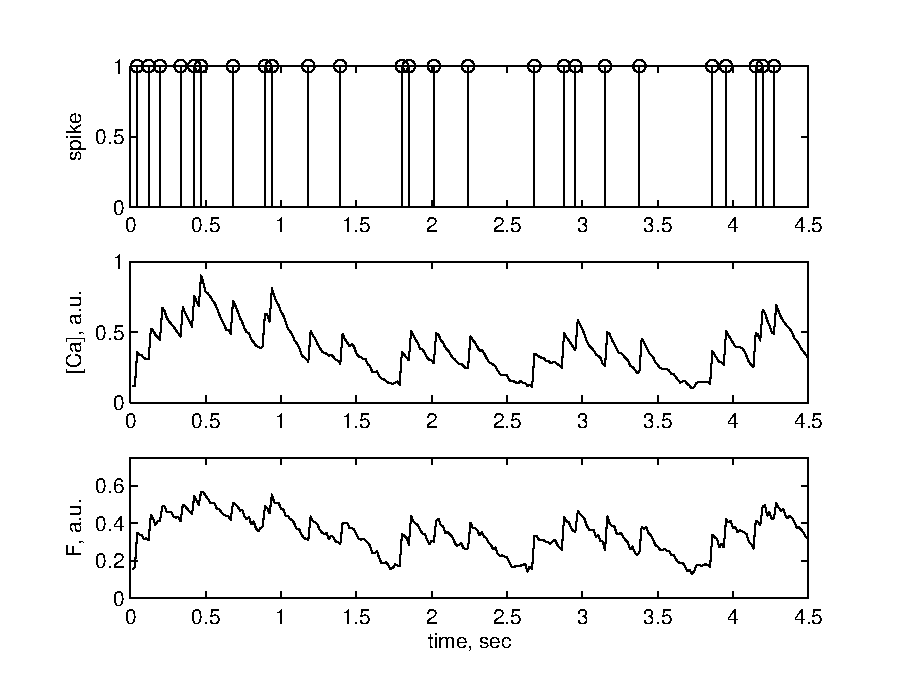
\includegraphics[width=250px]{Figure0a_fluor_eg_highSNR}
\end{minipage}
\caption{Examples of calcium and fluorescence traces for low (photon budget 5 Kph/neuron/frame, left)
and high SNR regimes (photon budget 40 Kph/neuron/frame, right).}
\label{fig:egfluor}
\end{figure}



\subsection{\label{sec:results:inference}Inference of the functional connectivity from the simulated calcium imaging data}
Connectivity matrix was calculated by solving maximum likelihood problem Eq.(\ref{eqn:likelihoodGLM-expl}). Specifically,
\begin{align}
\label{eqn:likelihoodGLMmoda}&E[\log P_{GLM}(n_i|{bf n}_{/i},W)]=\sum_t \left( n_i(t) \log J_i(t) - (1-n_i(t)) \exp(J_i(t)) \Delta \right),\\
\label{eqn:likelihoodGLMmodb}&J_i(t)=b_0^i+\sum\limits_j \sum\limits_{t'<t} w_{ij}(t-t')n_{j}(t')=
b_0^i+\sum\limits_j w^{ij}_s \sum\limits_{t'<t} \exp(-(t-t')/\tau_h)n_j(t').
\end{align}
The sum in Eqs.(\ref{eqn:likelihoodGLMmoda}) and (\ref{eqn:likelihoodGLMmodb}) was over the sample of $\{n_i(t)\}$ and over the time-bins $t'$ discretized at the time steps $\Delta$ corresponding to the calcium imaging frame rates of either 33Hz (30 ms) or 66Hz (15 ms). The coincident time bin $t=t'$ was not used in Eqs.(\ref{eqn:likelihoodGLMmoda}), (\ref{eqn:likelihoodGLMmodb}), i.e.
all spike pairs within same time-frame were removed from the GLM fit.
Because time position of spikes inferred from fluorescence data typically had inaccuracy $\sim \Delta$, temporal order of such closely positioned spike pairs could be confused in the sample ${\bf n}$, thus, polluting GLM dataset.
E.g., given two neurons $i$ and $j$, if the number of spikes of neuron $i$ following neuron $j$ within $\Delta$ was $m_{ij}$, while such in the reverse order was $m_{ji}$, the difference $\Delta m = m_{ij}-m_{ji}$ effectively corresponded to the difference in GLM weights $w_{ij}-w_{ji}$. However, if during spike inference the order of such spikes was confused with probability $p\approx 1/2$, the observed number of spike pairs $ij$ would become $m_{ij}(1-p)+m_{ji}p$, while for the reverse order this would be $m_{ji}(1-p)+m_{ij}p$. The difference would thus drop to $\Delta m '= (1-2p)\Delta m$ with the variance remaining the same. This effect complicated the problem of estimating functional connectivity $W$ by effectively mixing $w_{ij}$ and $w_{ji}$ and introducing large error in $W$ estimate moving it toward the symmetrized version of $W$.

Since the connectivity weights $w_{ij}(t)$ were time-dependent, to compare inferred and true connectivity we introduced a "scalar" version of the connectivity matrix defined via the peak values of EPSP/IPSP at each connection, i.e. the scalar connection weights were $w^{ij}_s=\text{sign}(w_{ij})\max_{t} |w_{ij}(t)|$.
If the time dependence of $w_{ij}(t)$ was assumed to be unknown, the first equation in (\ref{eqn:likelihoodGLMmodb}) was used to correlate $n_i(t)$ with $n_j(t')$ for $t'<t$ up to given depth $m$.
Since each next term in Eq.(\ref{eqn:likelihoodGLMmodb}) was exponentially smaller than the previous one, we found that the best results were obtained assuming $m=1$, allowing for better results by reducing the number of unknowns for the same amount of data. 
For independent approximation below the time-dependence of $w_{ij}(t)$ was assumed to be "known" exponential, and the weights were estimated using reduced histories $h_{i}(t)=\sum_{t'<t} \exp(-(t-t')/\tau_h)n_{i}(t')$ with time constant $\tau_h=10$ ms. The scalar connection weights were directly estimated as $w^{ij}_s=w_{ij}(t=0)$.
Such inferred connectivity weights were then compared with true $w^{ij}_s$.

We shall note that because of coarse time discretization $\Delta \approx 15-30$ ms relative to EPSP/IPSP time scale of $\tau_w = 10-20$ ms, the first term in the sum (\ref{eqn:likelihoodGLMmodb}) measured in GLM was $w_{ij}(\Delta)\approx w^{ij}_s\exp(-\Delta/\tau_w)$, substantially smaller than $w^{ij}_s$. Time discretization thus resulted in estimated weights differing from the true connectivity by a factor of $\sim \langle \exp(-\Delta/\tau_w) \rangle$, where the average is understood over the spike pairs within two consecutive time-bins. In our simulations, we observed that this factor was a constant for same $\Delta$ and $\tau_w$ and different network sizes $N$. For $\Delta=15$ ms and $\tau_w\approx 10$ ms this factor was  $\approx 0.45$.
Note that where $\tau_w$ varied from neuron to neuron, this scaling factor as well as any mismatch in the time-scale $\tau_h$ of $h_i(t)$ and the true EPSP/IPSP time-constant $\tau_w$ introduced added variability in the estimated weights $w^{ij}_s$. However, we found such added variance in the estimates of $w^{ij}_s$ to be insignificant for simulations where $\tau_w$ was allowed to vary for up to 25\% (data not shown).

Scaling bias theoretically could be removed by performing estimation of spike trains with finely discretized time. However, we were not successful in performing this calculation as the amount of data necessary to overcome variation in $W$ introduced by disordering of closely spaced spike-pairs appeared to be well over $\approx 10$ min of data used for most of the calculations here. Such high-time-resolution samples of spike trains were also substantially more computationally expensive to obtain and work with. For these reasons we did not pursue this path further, although it may be of interest in the future.

After performing functional connectivity reconstruction using MCMC-Gibbs method, we repeated the reconstruction using independent approximation. We found that MCMC-Gibbs method did not provide noticeable improvement over the independent approximation for imaging regimes where sufficiently accurate connectivity matrix could be recovered, Figure \ref{fig:mcmc-iid}. We therefore concluded that the independent approximation was equivalent to exact MCMC-Gibbs method for the purpose of inferring connectivity from calcium imaging data for experimentally interesting regimes.

Since fluorescence data is generally acquired at low frame-rate, one of the main limitation for the connectivity inference from calcium imaging is time-resolution of the inferred spike trains. In order to determine the limits on reconstruction due to this constraint, we compared weights inferred from fluorescence data with such computed from the true spike trains down-sampled at frame-rate of 33Hz or 66Hz. This served as a baseline for the "best" connectivity matrix reconstructions. We observed that baseline performance could be achieved from calcium imaging data, Figure \ref{fig:iid-base}.
Also, the same analysis of baseline performance showed that calcium imaging rates below 30Hz are generally insufficient for the purpose of inferring connectivity, Figure XXX.
\begin{figure}
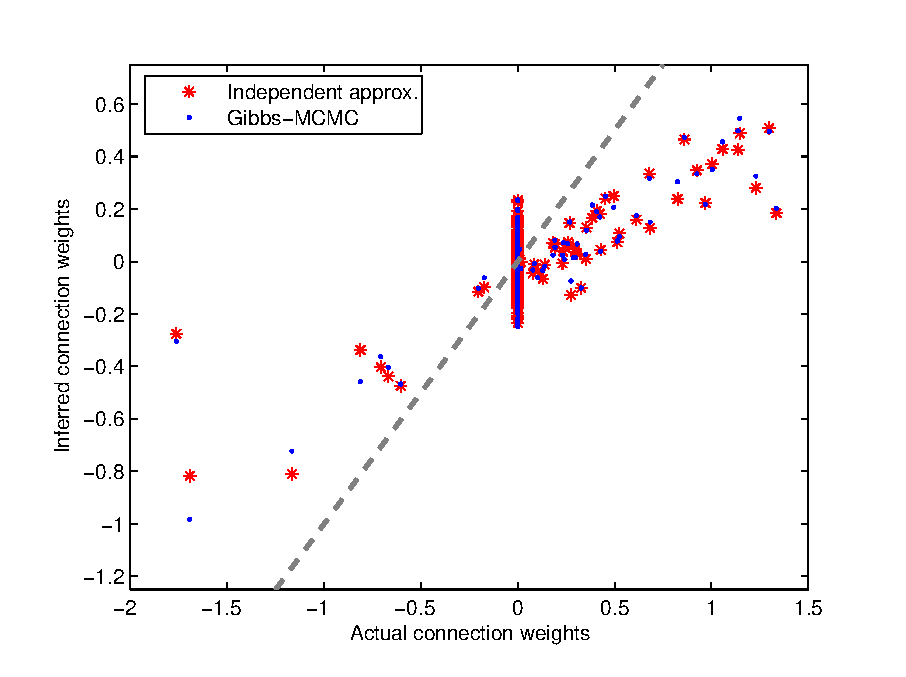
\includegraphics[width=275px]{Figure1_fluor_mcmc_vs_iid}
\caption{A scatter plot of inferred connectivity weights vs. real connectivity weights
using hybrid MCMC-Gibbs sampler and independent approximation, for a network of $N=25$ neurons imaged
with intermediate SNR ($10$ Kph/neuron/frame, see Figure \ref{fig:ca-noise} below); $r^2=0.48$ for MCMC-Gibbs and
$r^2=0.47$ for IID. Note that the connectivity weights thus inferred are nearly equal, thus showing that independent approximation is sufficient here for the purposes of estimating the connectivity matrix. Note also constant time-discretization scaling bias in the estimated weights due to missing proximal spike pairs.}
\label{fig:mcmc-iid}
\end{figure}
\begin{figure}
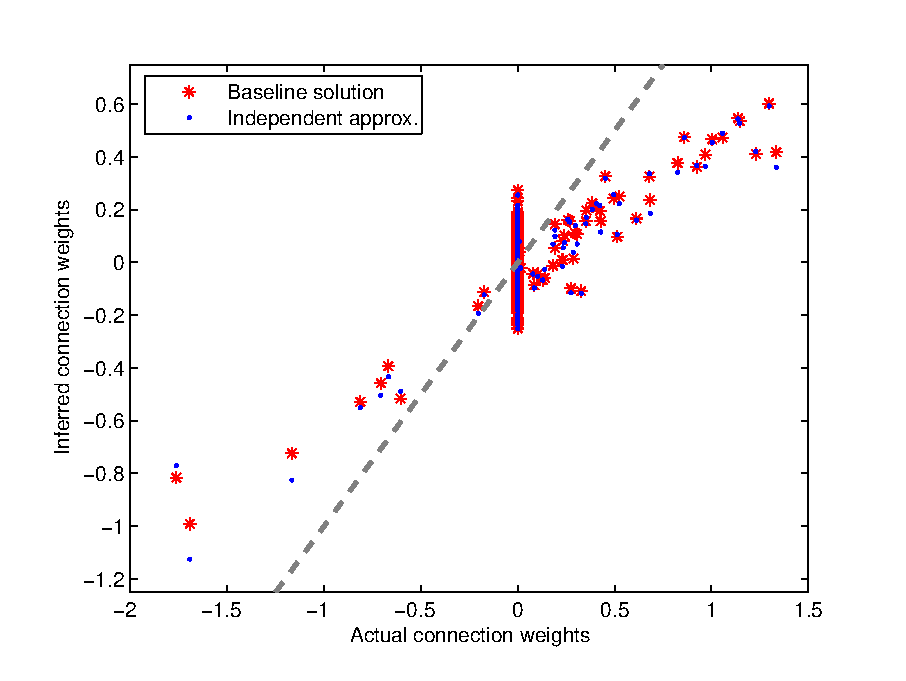
\includegraphics[width=275px]{Figure2_fluor_base_vs_iid}
\caption{A scatter plot of inferred connectivity weights vs. real connectivity weights
using independent approximation and true spike trains down-sampled to the frame-rate,
for a network of $N=25$ neurons imaged
with high SNR (40 Kph/neuron/frame, see Figure \ref{fig:ca-noise} below); $r^2=0.57$ for IID and $r^2=0.57$ for the baseline. Note that for sufficient SNR, the connectivity weights inferred from fluorescence data are nearly equal to such inferred from down-sampled true spikes, thus showing that calcium imaging is capable of achieving accuracy of spike extraction equivalent to direct observation of spike trains.}
\label{fig:iid-base}
\end{figure}
\begin{figure}
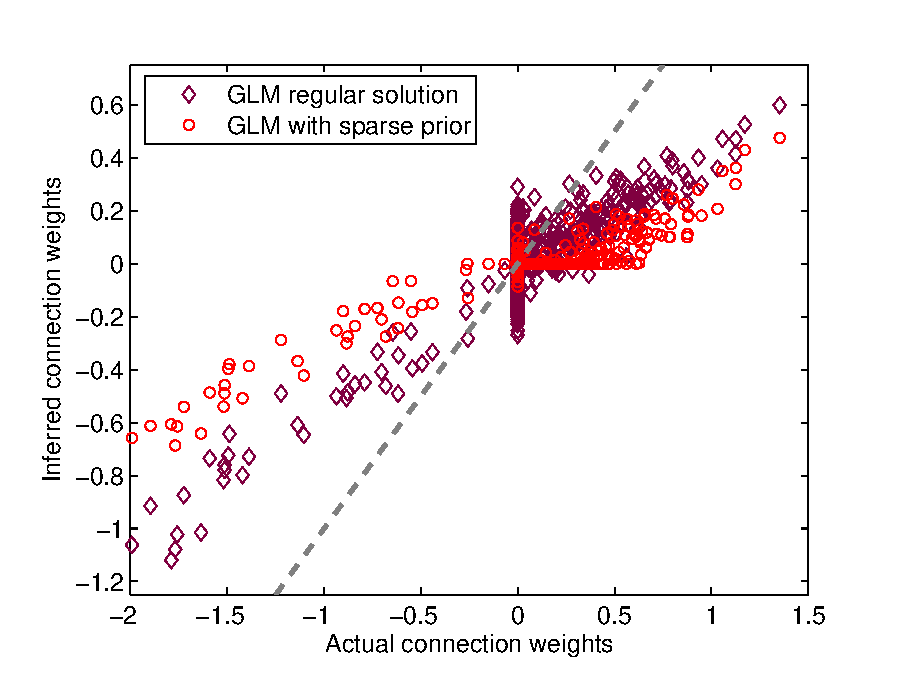
\includegraphics[width=275px]{Figure9_fluor_sparse_sol}
\caption{A scatter plot of inferred connectivity weights vs. real connectivity weights
using independent approximation and either GLM or sparse-prior GLM,
for a network of $N=50$ neurons imaged for $T=800$ s
with high SNR (40 Kph/neuron/frame, see Figure \ref{fig:ca-noise} below); $r^2=0.66$ for GLM solution and $r^2=0.85$ for sparse-prior GLM solution. Note that use of sparse prior allows to obtain significantly better approximation to the true connectivity matrix, although additional scaling bias is introduced in the estimate.}
\label{fig:sparse-sol}
\end{figure}

[ANOTHER FIGURE 30Hz]

We then considered the question what calcium imaging SNR was required to achieve time-resolution performance limits, particularly as determined by the photon budget of the experimental setup. Photon budget is defined here as the average count of photons collected by the detector from single neuron per single frame. It is experimentally determined by the factors such as dye quantum efficiency, excitation laser power, detector efficiency, microscope scanning speed, etc. Photon budget was one of the primary factors determining possibility of analyzing spike trains from calcium imaging data (the other key factors being frame-rate and neuron peak spike rate).
As should be expected, when amount of noise was high (low photon budget), inference from calcium imaging data was far below the baseline level, and with increasing SNR the baseline level was recovered. The SNR level necessary to achieve baseline performance was 20-40 Kph/neuron/frame, Figure \ref{fig:ca-noise}.
For comparison, from our experience with the analysis of real cells \cite{Vogelstein2009}, the photon budget in real data was $\sim 10$ Kph/cell/frame for in-vivo data collected at 15 Hz and $\sim 100$ Kph/cell/frame for in-vitro data at the same frame-rate.
\begin{figure}
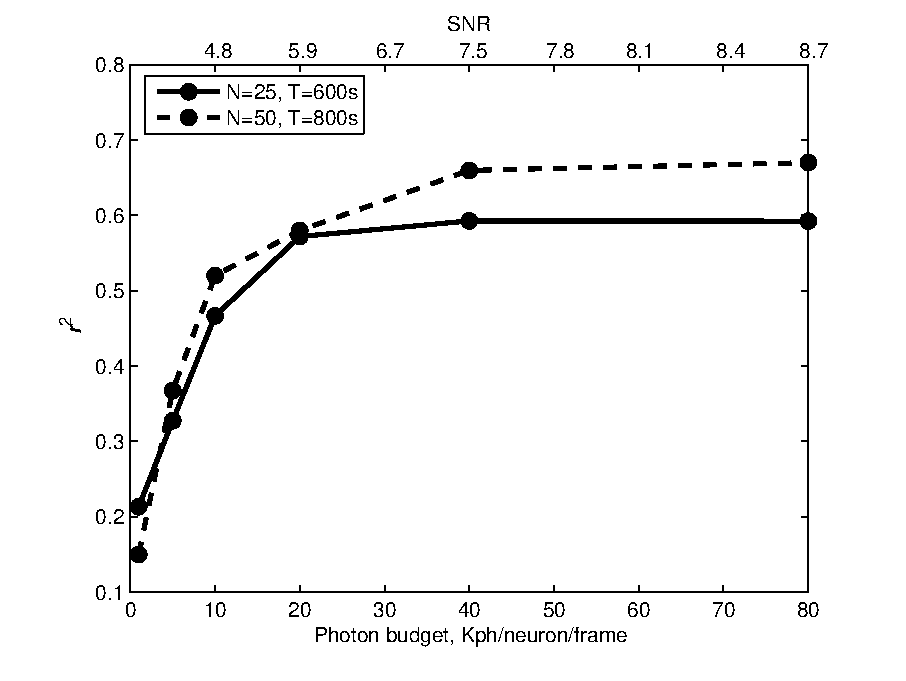
\includegraphics[width=275px]{Figure3_perf_vs_gamma}
\caption{Accuracy of inferred connectivity weights as function of noise amount in
calcium imaging data, as measured by photon budget per neuron-frame and fluorescence
signal to noise ratio
SNR=$\left({E[\Delta F^2 | \text{spk}]}/{E[\Delta F^2|\text{nospk}]}\right)^{1/2}$,
for networks of $N=25$ and $N=50$ neurons. Note that the photon counts on the order of 20-40 Kph/frame/neuron are required in order to achieve best reconstructions.}
\label{fig:ca-noise}
\end{figure}

In all cases we found that taking into account sparseness prior resulted in dramatic improvement in the inferred connectivity matrix, allowing to achieve for $T\sim 10$ min the same level of accuracy that would otherwise require over $T\sim 1$ hour of calcium imaging data (Figure \ref{fig:sparse-sol} and \ref{fig:data-time}). We also explored impact of the Dale's prior and found that improvement in the inferred weights there were much less significant, on the order of $10\%$ in the correlation coefficient $r^2$. If sparseness of the solution was previously accounted for, accounting for Dale's law led to no improvement in the result (Figure \ref{fig:data-time}).

We finally explored the question how much data was required for given reconstruction accuracy. First, we considered different observation times $T$, see Figure \ref{fig:data-time}. The observation time necessary to achieve $r^2$=0.5 was $T\sim 10$ minutes, while with GLM solver using sparse prior $r^2>0.6$ was achieved already at $T\sim 5$ minutes of calcium imaging. In agreement with the theoretical analysis of the Fisher information matrix in the Methods, the accuracy of the reconstruction did not depend on the size of the neural network inferred, see Figure \ref{fig:data-n}. Good reconstructions for $N=20-200$ could be obtained in all cases with $T\sim 10-30$ min of data. We conclude therefore that the connectivity could be successfully inferred from calcium imaging data, Figures \ref{fig:sparse-sol}, \ref{fig:distr} and \ref{fig:data-time}).

"Anatomical" connectivity could be recovered despite potential problems such as common input from correlated neurons, etc. This is owing to the particular form of the activity in our neural network, whereas firing of neurons occurred independently, thus, allowing GLM explore full range of possible input configurations and disentangle potential common inputs.
Estimation of the functional connectivity is fundamentally routed in observing changes in the spike rates conditioned on the state of the other neurons. Intuitively, such estimation can be compared to observing changes in $p({\bf n}(t))=\exp(\sum_j w_{ij}n_j(t))$ for different neural configurations ${\bf n}(t)$ or, equivalently, estimating vector ${\bf w}_i$ by observing a number of dot-products ${\bf w}_i {\bf n}(t)$ with different vectors ${\bf n}(t)$. Obviously, in order to be able to properly estimate all components of ${\bf w}_i$ the set of available ${\bf n}(t)$ should be rich enough to span all $N$ dimensions of ${\bf w}_i$. In case of independent firing such condition of "full dimensionality" is clearly satisfied.
Should this condition be violated, however, e.g. due to high correlation between spiking of few neurons, spike trains will not necessarily provide access to complete anatomical connectivity vector ${\bf w}_i$, and so the connection weights from the neurons providing correlated input may be "aggregated" into a single weight, split arbitrarily into a linear combination of weights, etc.

To test this effect we performed simulation of a hypothetical strongly coupled  neural network, still with unstructured random sparse connectivity now consisting additionally of strong component. Strong connections component was chosen to dynamically build up the actual firing rate to $\approx 5$ Hz from the base rate low $r=\exp(b^i_0)\approx 1$ Hz. Such strongly coupled network showed patterns of firing very different from weakly coupled networks considered above, Figure \ref{fig:rasters}.
In particular, large number of highly correlated, synchronously locked firings of many neurons were evident in this network.
Likewise, GLM was not able to identify the true connectivity matrix correctly, Figure \ref{fig:strongcouple}. 
\begin{figure}
\centering
\begin{minipage}[c]{0.45\hsize}
\includegraphics[width=250px]{Figure5a_hist_glm_vanilla}
\end{minipage}
\begin{minipage}[c]{0.45\hsize}
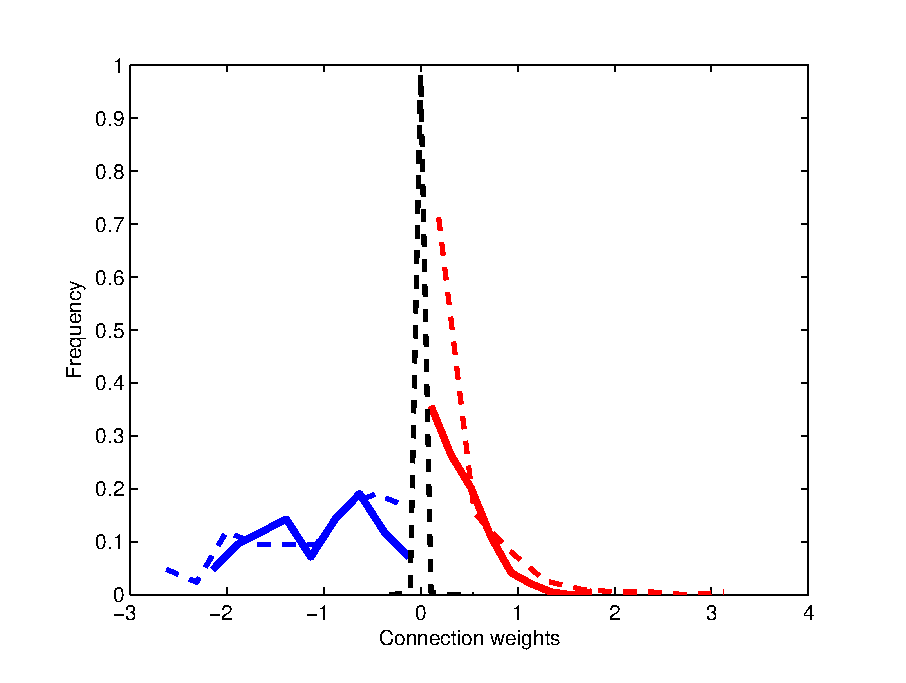
\includegraphics[width=250px]{Figure5b_hist_glm_sparse}
\end{minipage}
\caption{Distribution of connectivity weights inferred using calcium imaging, for
a network of $N=50$ neurons and $T=800$ s. The inferred distributions were rescaled
to have the same mean with the true distributions, owing the time-discretization scaling bias
discussed in the text.
Left panel is for GLM solution,
and right panel is for sparse-prior GLM solution.
Blue curves are for inhibitory connections, red curves are for excitatory
connections and black are for zero connections. Solid lines are original
distributions and dashed lines are inferred distributions. In GLM solution the quality of the inferred weights is certainly sufficient to say whether a pairs of neurons is connected, or whether given neuron is inhibitory or excitatory with high reliability; and such statements may be made from sparse-prior GLM solution almost with certainty.}
\label{fig:distr}
\end{figure}
\begin{figure}
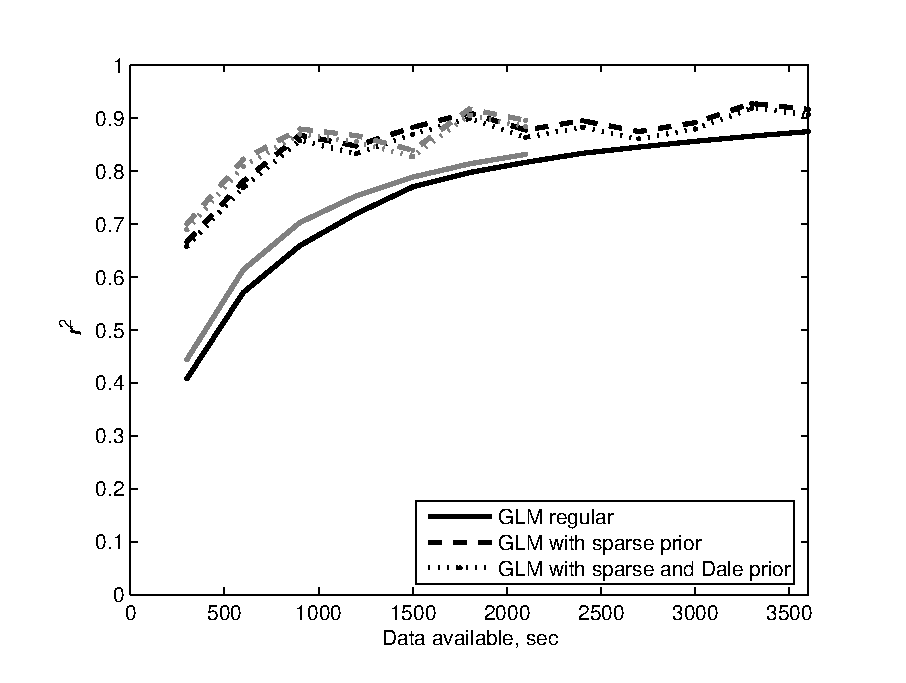
\includegraphics[width=275px]{Figure4_perf_vs_T}
\caption{Baseline accuracy of connectivity weights inference as the function of imaging time. Black lines are for $N=50$ and gray lines are for $N=100$. Note that accuracy does not depend on the number of neurons $N$, as shown in the Methods. Also, about 30 minutes of imaging time are sufficient for accurate estimation of the connectivity matrix using GLM solution, while the same accuracy of the reconstruction may be achieved with sparse-prior GLM solver already for 300-600 seconds of calcium imaging.}
\label{fig:data-time}
\end{figure}
\begin{figure}
\centering
\begin{minipage}[c]{0.45\hsize}
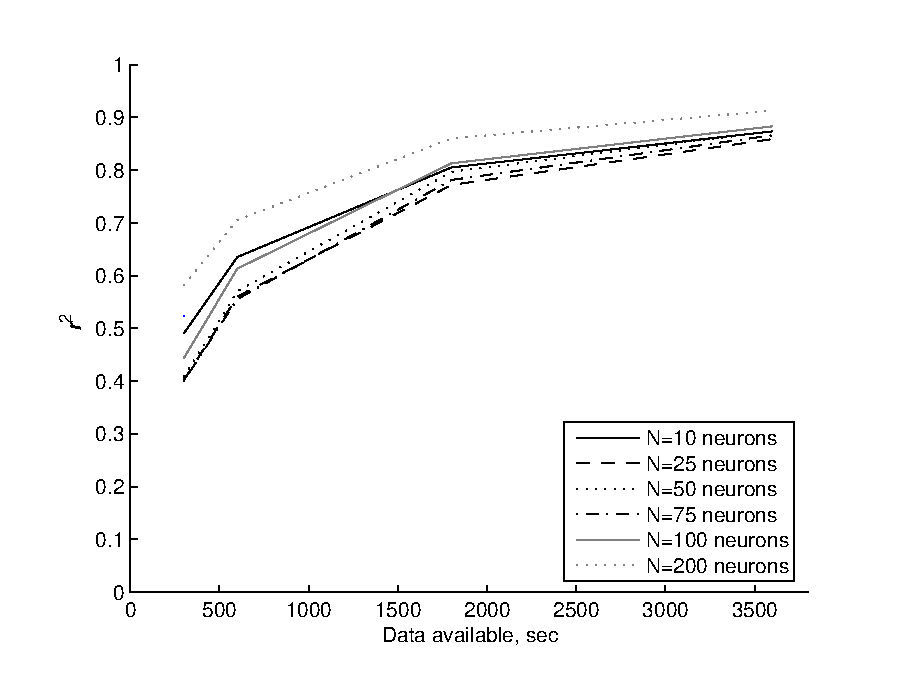
\includegraphics[width=250px]{Figure6a_perf_vs_N}
\end{minipage}
\begin{minipage}[c]{0.45\hsize}
\includegraphics[width=250px]{Figure6b_perf_vs_N_sparse}
\end{minipage}
\caption{Baseline accuracy of connectivity weights inference for
for networks of different size from $N=10$ to $N=200$ neurons.
Accuracy does not depend on the number of neurons $N$ in agreement with theoretical analysis in Methods. 300-600 seconds of calcium imaging data are sufficient for estimating connectivity matrix using sparse-prior GLM solver, and about 30 minutes of observations are sufficient using GLM solver.}
\label{fig:data-n}
\end{figure}
\begin{figure}
\centering
\begin{minipage}[c]{0.45\hsize}
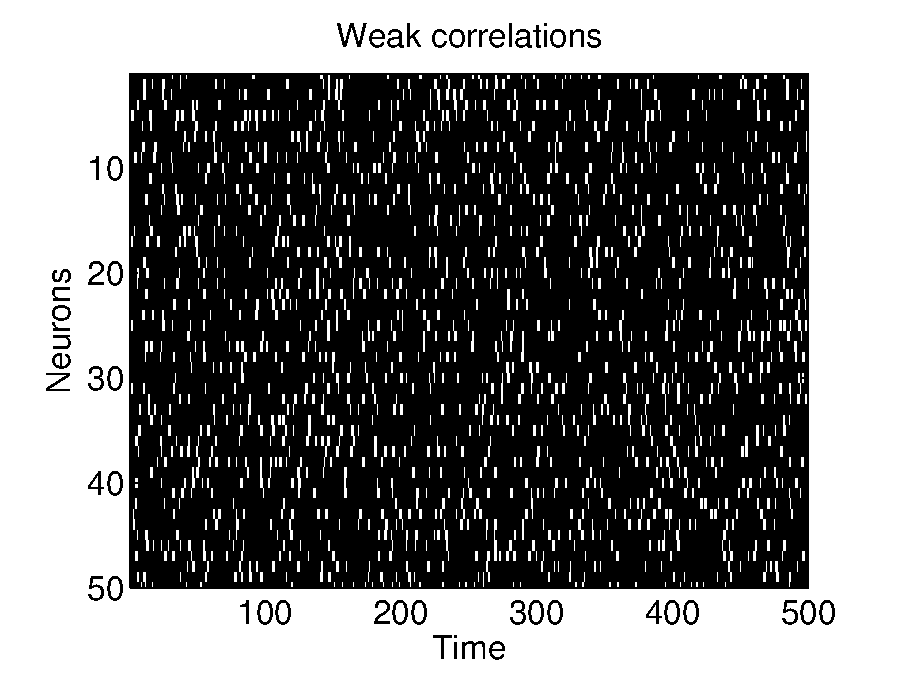
\includegraphics[width=250px]{Figure7b_raster_weak}
\end{minipage}
\begin{minipage}[c]{0.45\hsize}
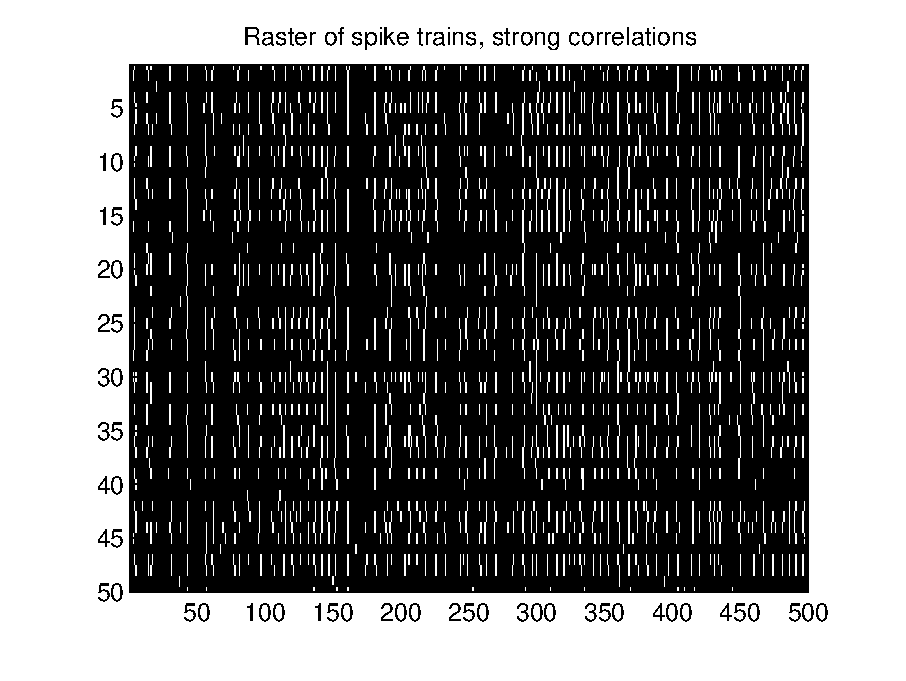
\includegraphics[width=250px]{Figure7a_raster_strong}
\end{minipage}
\caption{15 s of simulated spike trains for a weakly coupled (left)
and strongly coupled (right) stochastic networks. Note that in weakly coupled network spikes are sufficiently uncorrelated to allow access to all different neural connectivity configurations necessary to estimate complete anatomical connectivity vectors ${\bf w}_i$. In strongly coupled case many instances of highly synchronous locked firings are evident, thus reducing dimensionality of the observed dynamic space of the network, and preventing functional connectivity from faithfully representing anatomical connectivity.}
\label{fig:rasters}
\end{figure}
\begin{figure}
\centering
\begin{minipage}[c]{0.45\hsize}
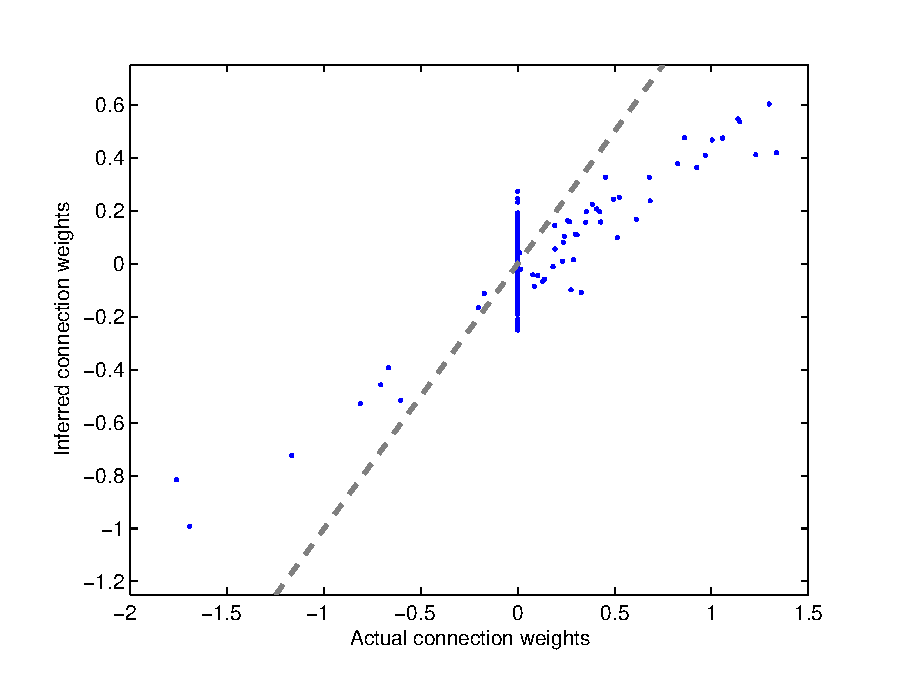
\includegraphics[width=250px]{Figure8b_fluor_weak_glm}
\end{minipage}
\begin{minipage}[c]{0.45\hsize}
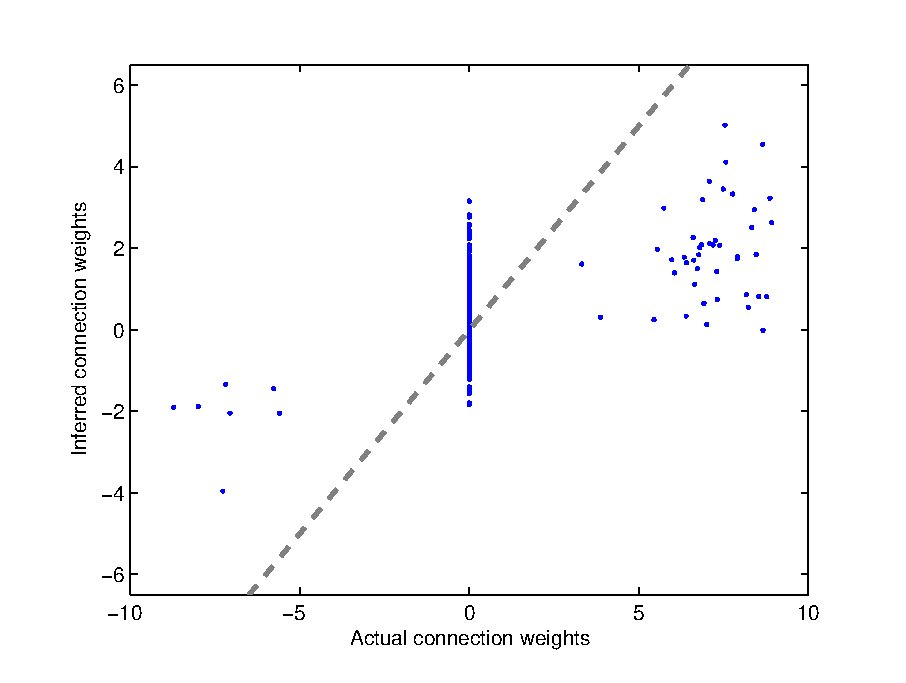
\includegraphics[width=250px]{Figure8a_fluor_strong_glm}
\end{minipage}
\caption{Baseline GLM solution for the connectivity matrix from 10 min of spiking data for weakly coupled network of $N=25$ neurons (left) and strongly coupled network (right). Note that GLM solution for strongly coupled neural network does not provide access to the structure of anatomical connectivity.}
\label{fig:strongcouple}
\end{figure}


\section{\label{discussion  }Discussion}
Functional connectivity may fail to faithfully represent anatomical circuit structure if false correlations are present between different neurons, induced e.g. by common inputs, or if the dynamics of neural population is entirely concentrated on a low-dimensional subspace of the full configurational space ${\bf n}$. Note that these two statements are, in a sense, stating the same condition: if activity of different neurons is tightly correlated, their dynamics is concentrated on a low-dimensional plane and vice-versa - concentration of dynamics onto a low-dimensional plane will be perceived as correlation in activity of different neurons. In turn, low dimensionality of the neural dynamics may be caused by different factors, including common input, small subset of command neurons driving the circuit, or even emergent property of a network. Low dimensionality of neural dynamics results in that the inference problem becomes underdetermined, i.e. there may exist directions in ${\bf w}_i$ along which connectivity is not constrained by neural activity data (i.e. directions orthogonal to the subspace of all observed neural activity configurations), or is poorly constrained. This, naturally, leads to ${\bf w}_i$ being poorly defined along these directions. The necessary condition for good correspondence between functional connectivity weights ${\bf w}_i$ and anatomical connectivity, therefore, is {\em full-dimensionality} of the observed set of neural configurations. In case of spontaneously firing system of neurons this condition is satisfied by many neuron-firings occurring independently, thus, allowing to fully sample all possible directions in ${\bf w}_i$.
Still, spontaneously active preparation by itself may fail to display sufficient degree of independence between firing of neurons due to low-dimensionality of observed activity space, e.g. because of emergent properties of the circuit. In that case necessary variety of independent neural activity patterns may be enforced by randomly activating subsets of neurons via ChR2 or glutamate uncaging.

We also note that the correlations induced by secondary and so on synaptic transmissions (such as when neuron $A$ results in firing of neuron $B$, which in turn results in firing by neuron $C$), are all properly resolved in GLM-fitting process via the so called explaining-away process. In other words, because we do not just identify correlations between neural firings with the functional connectivity weights $w_{ij}$, but instead statistically fit a model of neural interactions, if found weights between neurons $A$ and $B$, and $B$ and $C$ are sufficient to explain the correlation between $A$ and $C$, the weight connecting $A$ and $C$ will not appear in the model - the correlation between $A$ and $C$ was "explained away" by correlations between $A$ and $B$, and $B$ and $C$. By this, the multi-synaptic firing patterns do not confuse our estimation process.

ADD SOME RAVINGS ABOUT PROPER/IMPROPER FUNCTIONAL CONNECTIVITY.

\begin{acknowledgments}
Thank everyone for their help and support [Bows, Bows, Bows] !!!
\end{acknowledgments}

\bibliography{mybib}
\bibliographystyle{amsplain}

\end{document}
